\documentclass[12pt]{article}
\usepackage{amsmath}
\usepackage{amsfonts}
\usepackage{geometry}
\usepackage{graphicx}
\usepackage{setspace}
\usepackage{parskip}
\usepackage{hyperref}
\usepackage{graphicx}
\usepackage{float}

\geometry{a4paper, margin=1in}
\setstretch{1.2}

\title{Statistical Outlier Detection Notes}
\author{}
\date{}

\begin{document}

\maketitle

\section*{Outlier Detection Using Mean and Standard Deviation (Z-Score Based Outlier Detection)}

To detect outliers in a dataset $\Delta$, we use the mean and standard deviation:

\begin{itemize}
    \item $\mu(\Delta)$: Mean of the data
    \item $\sigma(\Delta)$: Standard deviation of the data
\end{itemize}

\subsection*{Normal Range}

The normal range is defined as:

\[
\mu(\Delta) \pm 2\sigma(\Delta)
\]

This means most data points (about 95\% if normally distributed) are expected to lie within this range.

\subsection*{Outlier Condition}

A value is considered an outlier if:

\[
\Delta < \mu(\Delta) - 2\sigma(\Delta) \quad \text{or} \quad \Delta > \mu(\Delta) + 2\sigma(\Delta)
\]



\begin{itemize}
    \item $\Delta$ - Orderbook Delta Depth of 5\% from Coinbase
    \item $\mu(\Delta)$ - Mean of $\Delta$
    \item $\sigma(\Delta)$ - Standard deviation of the dataset
\end{itemize}


\subsection*{Strength of Signal}

To not only detect outlier price points but also see how far they are expanded from the mean I use the Z-score for each data point being detected as an outliers
\newpage
The Z-score is calculated as:

\[
Z = \frac{\Delta_5 - \mu(\Delta_5)}{\sigma(\Delta_5)}
\]

Only points outside the $[\mu - 2\sigma, \mu + 2\sigma]$ interval are considered outliers.  
For these, the signal strength is defined as $|Z|$, indicating how extreme the value is compared to the distribution.

\textit{Example:}  
A point with a Z-score of $+3.1$ is a stronger signal than one at $+2.1$, since it is farther from the mean.  
Non-outliers receive a signal strength of 0. 
\footnote{Visualisation inside of Figure 1}





\begin{figure}
    \centering
    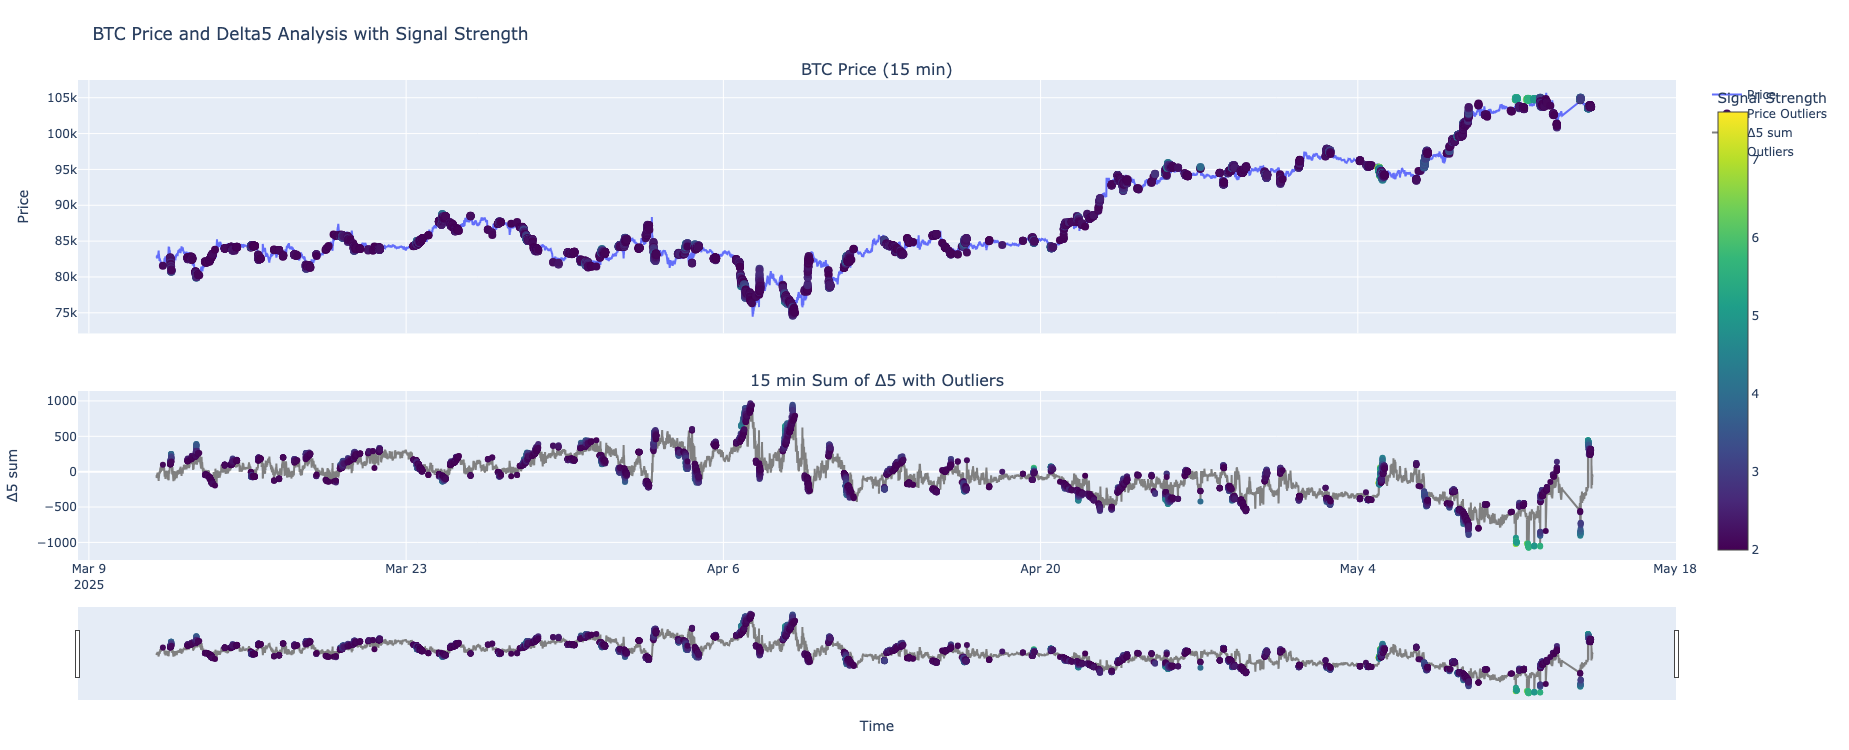
\includegraphics[width=1\textwidth]{imgs/outlier_signal_visualised.png}
    \caption{Heatmap Outlier}
\end{figure}




\newpage


\subsection*{Idea behind}

\begin{itemize}
    \item This method assumes data is roughly normally distributed.
    \item Using $2\sigma$ captures approximately 95\% of data points under a normal distribution.
    \item You can adjust the multiplier (e.g., $3\sigma$) for stricter or looser thresholds.
\end{itemize}


\begin{figure}
    \centering
    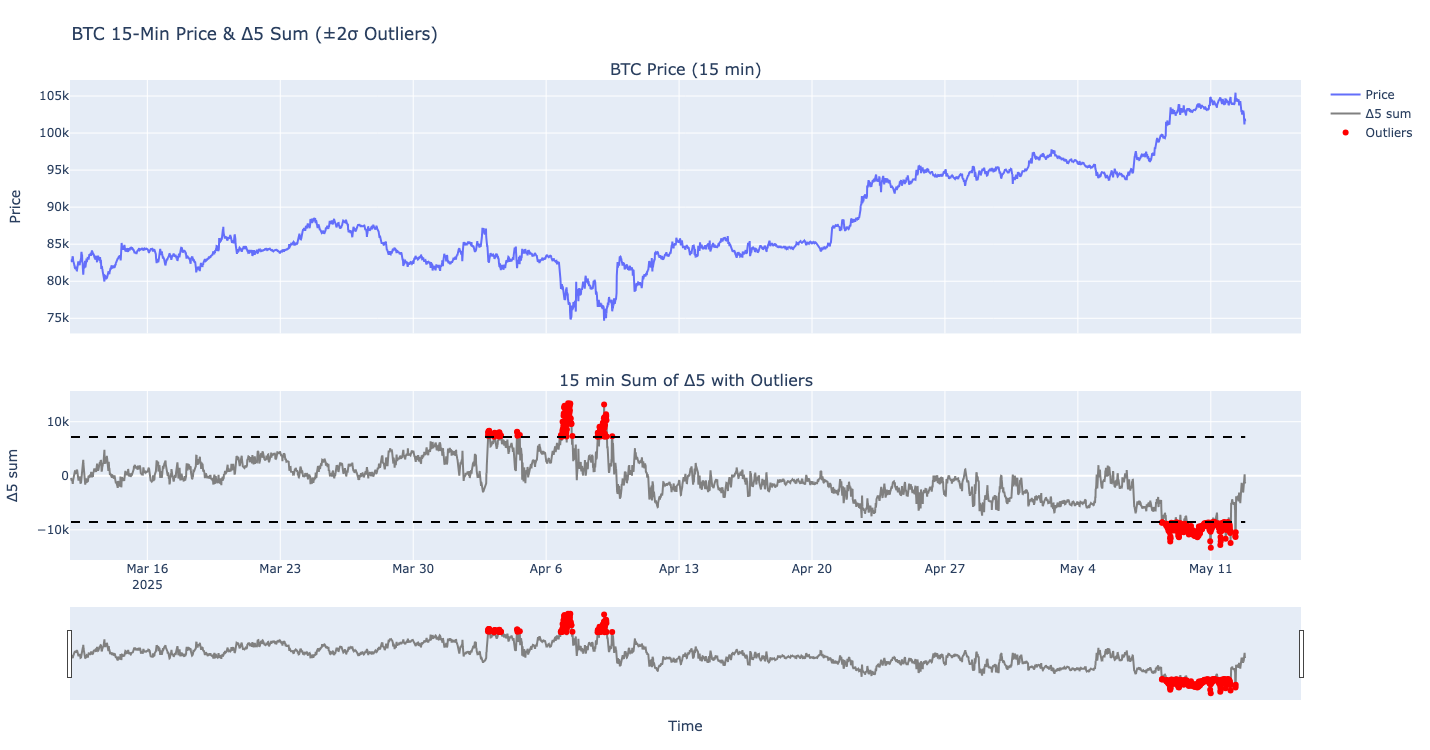
\includegraphics[width=1\textwidth]{imgs/ResultsOfSTDoutlierDecection.png}
    \caption{results over a two month data set}
\end{figure}


\subsection*{Future Plans}

\begin{itemize}
    \item Test on more data
    \item use rolling windows (e.g. 1 day or 1 week) for local context.
    \item Compare sensitivity with +- 1.5$\sigma$ or +-2.5$\sigma$
\end{itemize}

\newpage

\subsection*{Order Book Delta RSI (14-period)}

The Relative Strength Index (RSI) applied to the order book delta $\Delta$ is defined as:

\[
\text{RSI}_{\Delta}(t) = 100 - \frac{100}{1 + RS(t)}
\]

where

\[
RS(t) = \frac{\text{Average Gain over 14 periods}}{\text{Average Loss over 14 periods}}
\]


\subsubsection*{Dictionary of Terms}

\begin{itemize}
  \item $\Delta(t)$ — Order book delta at time $t$ (e.g., 5\% depth imbalance)
  \item $\text{Gain}$ — Positive change in $\Delta$: $\Delta(t) - \Delta(t-1) > 0$

\end{itemize}

\begin{figure}[H]
    \centering
    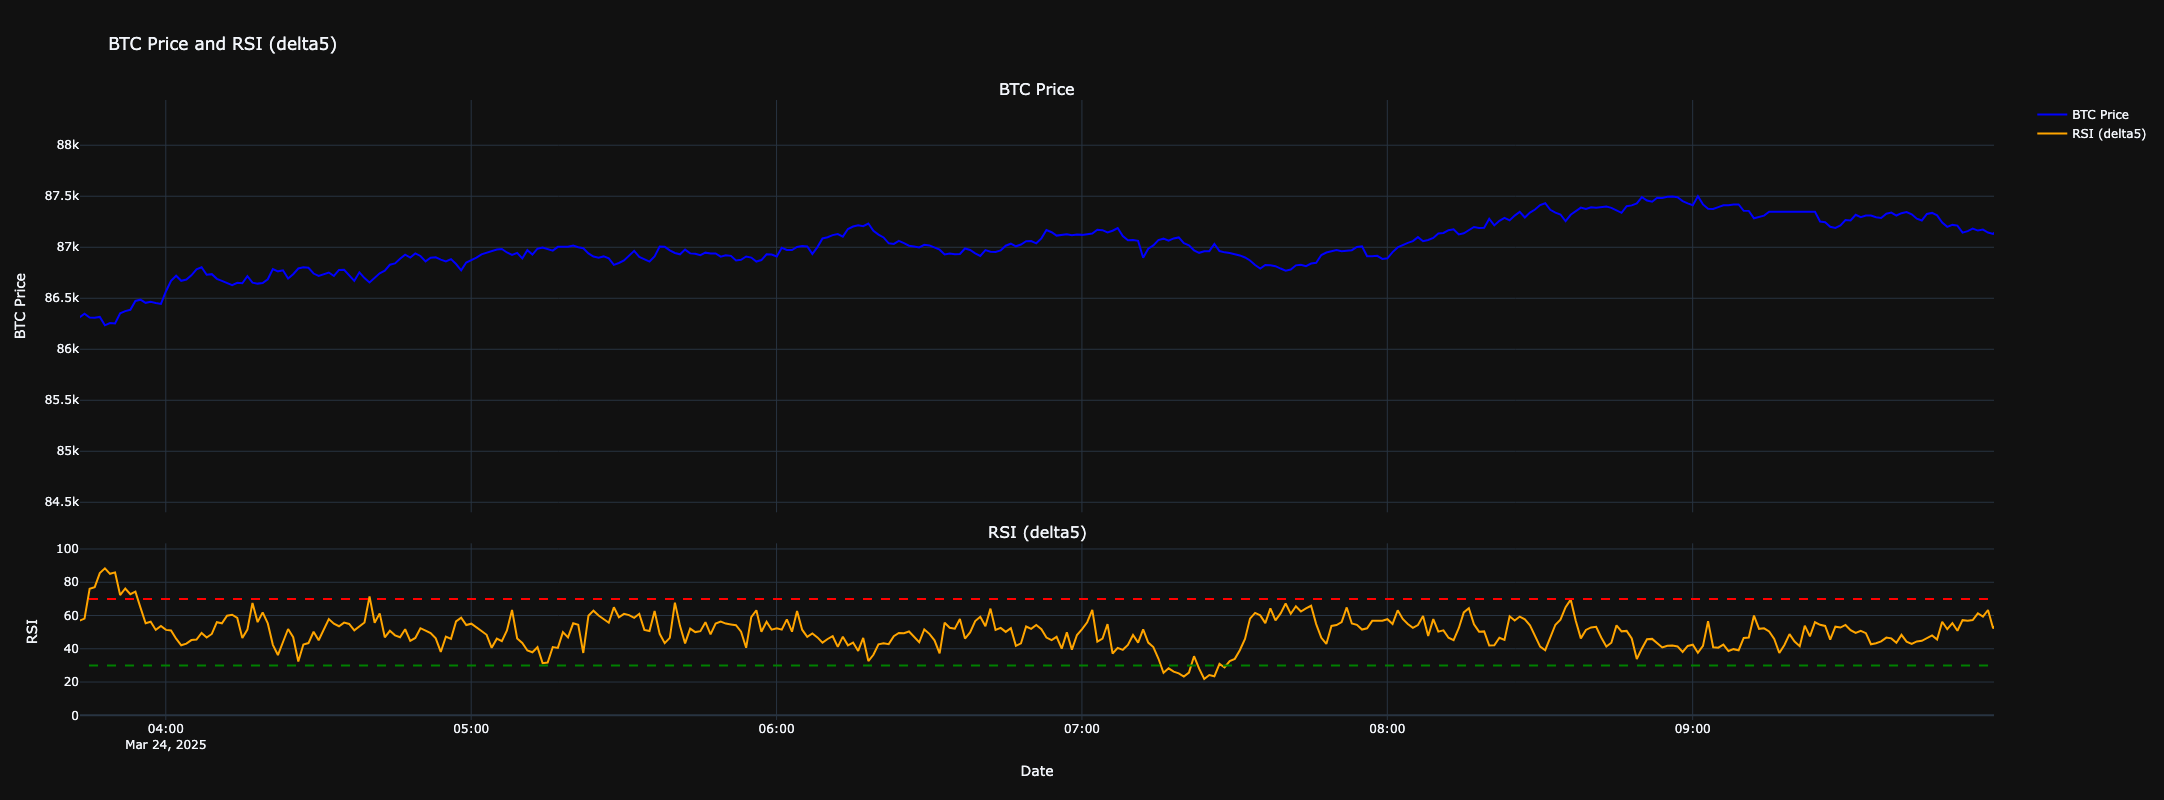
\includegraphics[width=0.8\textwidth]{imgs/RSI1min.png}
    \caption{1 min time frame RSI orderbook depth 5\%}    
\end{figure}
\begin{figure}[H]
    \centering
    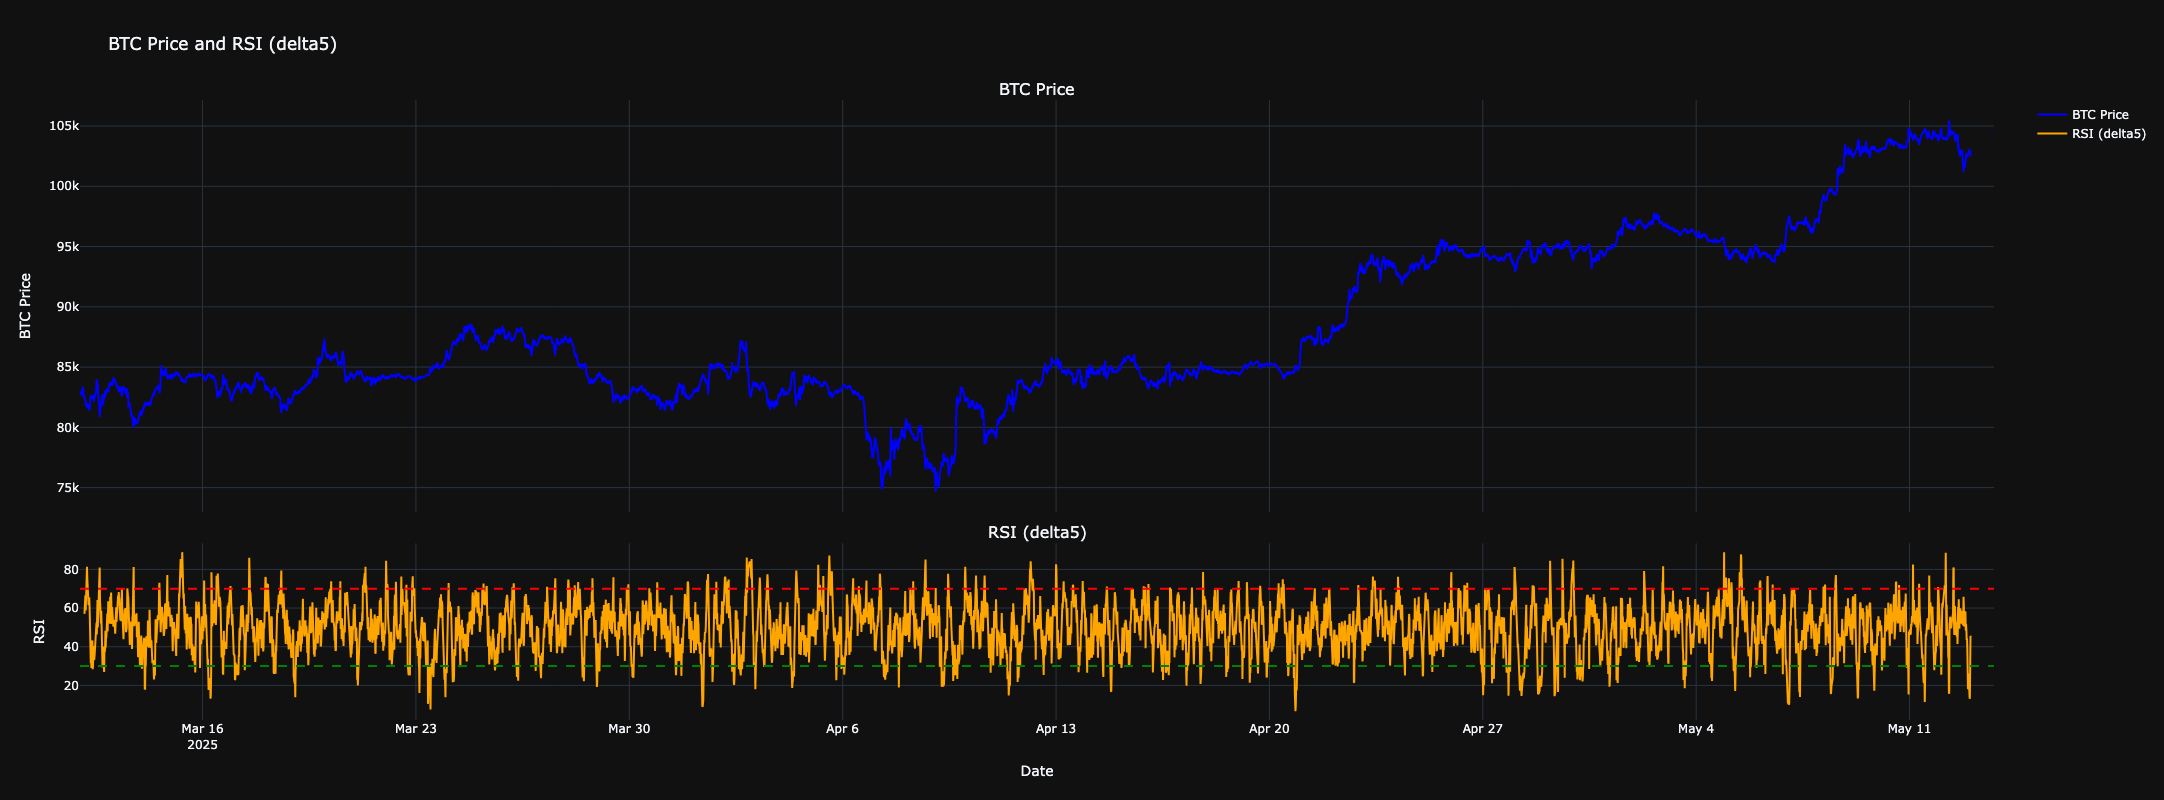
\includegraphics[width=0.8\textwidth]{imgs/15minRsi.png}
    \caption{15 min time frame RSI orderbook depth 5\%}
\end{figure}

\begin{figure}[H]
    \centering
    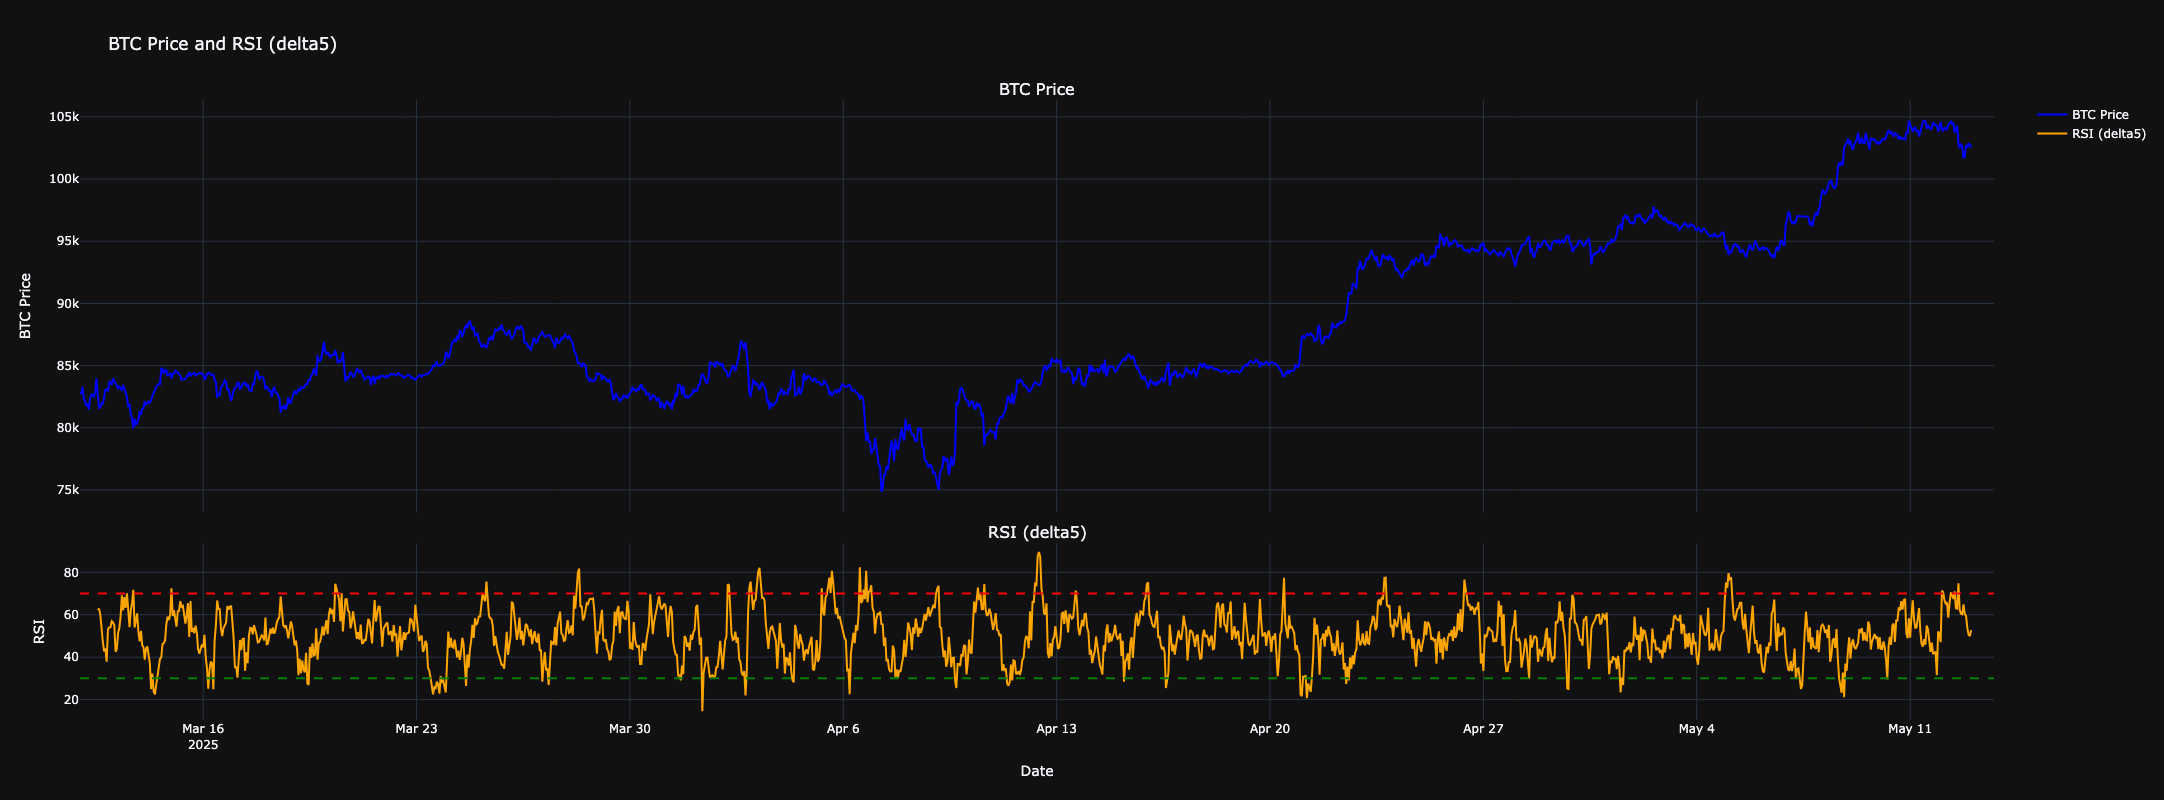
\includegraphics[width=0.8\textwidth]{imgs/60minRSI.png}
    \caption{60 min time frame RSI orderbook depth 5\%}
\end{figure}




\section*{EMA compression/expanssion}


\end{document}